This thesis uses the ICOLMDZOR limited area model (LAM) to study the impacts of simulated irrigation on the atmosphere and the water cycle. This model relies on the atmosphere (ICOLMDZ) and land surface (ORCHIDEE) components of the IPSL-CM in its latest version. 
Historically, the LMD General Circulation Model was first developed with a regular longitude-latitude grid \citep{sadourny_laval_1984}, before introducing the zoom capability \citep{li_ensemble_1999} which led to the name LMDZ. 
A land surface scheme named SECHIBA, was introduced in \citet{ducoudre_sechiba_1993} to represent water and energy budgets on continental surfaces. 
IPSL was founded in 1995 and the LMD GCM became part of the IPSL-CM1 where it was coupled to an ocean and sea ice model \citep{braconnot_adjustment_1997}.
Later, the IPSL-CM4 contributed to the third phase of the Coupled Model Intercomparison Project (CMIP3) with simulations using LMDZ4 \citep{hourdin_lmdz4_2006} and the land surface model (LSM) ORCHIDEE \citep{krinner_dynamic_2005}, largely based on the aforementioned surface scheme of LMDZ.
Two versions of the IPSL-CM5 contributed to CMIP5, including one with a new version of the atmospheric physics, LMDZ5B \citep{hourdin_lmdz5b_2013}.
For CMIP6, the model evolved into IPSL-CM6-LR \citep{boucher_presentation_2020}, with a new version of the atmospheric GCM, LMDZ6A \citep{hourdin_lmdz6a_2020}, and of the LSM, ORCHIDEE 2.0 \citep{cheruy_improved_2020}. 
While preparing CMIP7, the IPSL-CM is undergoing a major evolution in its atmospheric component by changing to a new dynamical core, DYNAMICO \citep{dubos_dynamico-10_2015}, which uses an icosahedral grid instead of a regular longitude-latitude discretization. Within IPSL-CM7, which is still under development, the atmospheric component is now called ICOLMDZ, and its association with ORCHIDEE is referred to as ICOLMDZOR. Although a new version of the physics scheme is expected to be integrated into IPSL-CM7, ICOLMDZ can also function with the pre-existing physics of LMDZ, as was the case for the present work. 
Coincidentally with the development of DYNAMICO, a new functionality was implemented, to run ICOLMDZOR as a LAM, unlocking new perspectives in regional modelling with the IPSL-CM. 

Section \ref{sec:ORCHIDEE} first presents the version of the ORCHIDEE LSM used, with a special focus on the most relevant processes for this work such as the water and energy budgets, river routing and irrigation. 
Section \ref{sec:ICOLMDZLAM} describes the ICOLMDZ LAM, and Section \ref{sec:sim_setups} details the simulations setups used for these coupled simulations. 
Finally, the evaluation datasets used in this thesis are presented in Section \ref{sec:eval_datasets}.

\section{ORCHIDEE land surface model}
\label{sec:ORCHIDEE}
\subsection{General structure}
ORCHIDEE (Organizing Carbon and Hydrology In Dynamic EcosystEms) is a land surface model (LSM). Various "branches" and versions exist within the model, as the base structure presented in \citet{krinner_dynamic_2005} has been adapted and extended to meet different research objectives. 
This PhD work uses branch 2.2 which is similar to the ORCHIDEE 2.0 model used in CMIP6 \citep{cheruy_improved_2020, boucher_presentation_2020} but for minor bug corrections. It also includes a global irrigation scheme that was recently developed and evaluated \citep{arboleda-obando_validation_2024}. While the version chosen for CMIP7 simulations is ORCHIDEE v4.2, which integrates recent developments for the modelling of snow, permafrost, vegetation, carbon, nitrogen and phosphorus cycles, branch 2.2 is still used for developments focused on surface hydrology, that can later be introduced in other branches.
%Coupling with an atmosphere and ocean model imposes significant computational constraints, leading to the simplification or omission of certain processes for global climate simulations.
The following description of this model version is partly based on two PhD theses \citep{campoy_influence_2013,arboleda-obando_feedback_2023}.

\hfill

ORCHIDEE v2.2 contains several modules:
\begin{itemize}
    \item SECHIBA \citep[\textit{Schématisation des Échanges Hydriques à l’Interface entre la Biosphère et l’Atmo\-sphère}][]{ducoudre_sechiba_1993}. Initially developed as the surface scheme of the LMDZ GCM, this module computes surface energy and water budgets, including interactions with the atmosphere. As detailed in section \ref{sec:water}, it models vertical infiltration and redistribution of water into the soil, as well as horizontal transfers through the river network.
    \item STOMATE \citep{krinner_dynamic_2005}. This module simulates biological surface processes such as photosynthesis and phenology evolution, enabling the representation of seasonal variations in leaf area index (LAI), and thus evapotranspiration.
    \item LPJ \citep{sitch_evaluation_2003}. This optional module describes the long-term evolution of vegetation to represent land use adaptation to climate, but it is not capable of representing fast evolutions of land use induced by human activities. Therefore, in this work, this module is inactive, and vegetation evolution is instead prescribed using annual land-cover maps described in Section \ref{sec:ORCH_input_data}.
\end{itemize}

\subsection{Atmospheric forcing}
ORCHIDEE can interface with the atmosphere in either offline mode (also called forced) or coupled mode. The simulation domain is discretized into grid cells, with a resolution that follows the atmospheric forcing or the grid of the coupled atmospheric model.
In the first case, a meteorological forcing (typically obtained from a bias-corrected reanalysis) provides values for downward radiation (shortwave and longwave), precipitation (rain and snow), air temperature and specific humidity at 2 m, wind speed at 10 m (eastward and northward components), and surface pressure. 
In the second case, ORCHIDEE is coupled with an atmospheric model that calculates these variables in real time while receiving certain variables computed by ORCHIDEE (surface roughness, albedo, turbulent fluxes, surface temperature). ORCHIDEE's time step also adapts to the forcing, usually 30 minutes in oflline simulations, and is the same as the atmospheric physics when coupled (15 minutes for LMDZ).
Within the IPSL climate model, ORCHIDEE can be coupled with the atmospheric model ICOLMDZ in a standard configuration called ICOLMDZOR using a semi-implicit coupling scheme described in Section \ref{sec:energy}.

\subsection{Input data}
\label{sec:ORCH_input_data}
In addition to meteorological variables, the LSM requires input data that describe the continental surface. 

Each grid cell must be assigned a soil texture which determines various hydrological and thermal soil parameters. 
For CMIP6 simulations, the map from \citet{zobler87802world} was used to assign the dominant texture in each grid cell, with a resolution of 1°. 
This map was used for the offline simulations of Chapter \ref{chap:routing}
whereas the coupled simulations of Chapters \ref{chap:monthly}, the dominant USDA texture was obtained from the map of \citet{reynolds_estimating_2000}, which has a resolution of 5 arcmin and distinguishes 12 soil textures.

To characterize vegetation, ORCHIDEE v2.2 defines 15 Plant Functional Types (PFTs), each associated with a set of characteristic parameters used to compute their average height, leaf area index (LAI), and albedo. 
The fraction of each PFT in a grid cell is obtained from annual input maps derived from the Medium Resolution (300\,m) Land Cover product from the Climate Change Initiative (CCI) of the European Space Agency (ESA) \citep{bontemps_multi-year_2015}, and the Land Use Harmonization dataset \citep[LUH, ][]{hurtt_harmonization_2020} with the method described in \citet{lurton_implementation_2020}.
The offline simulations of Chapter \ref{chap:routing} use 0.25° resolution maps, whereas the coupled simulations in Chapter \ref{chap:monthly} and \ref{chap:liaise} use 0.1° resolution input maps. These maps change annually until 2014 and the PFT map was frozen to 2014 for the rest of the simulations (2015-2022).
For future climate simulations presented in \ref{sec:climate_change} the PFT maps were extended following the SSP5-8.5 scenario.

Each grid cell is divided into three tiles with distinct soil columns for subsurface hydrology, grouping multiple PFTs: one for bare soil, one for trees, and one for low vegetation (crops and grasses), as shown in Fig. \ref{fig:ORC_discretization} and \ref{fig:water_balance_AD}. 
Although they share the same soil texture within a grid cell, these columns were 
defined with independent water budgets to avoid large trees from extracting unrealistic amounts of moisture from the soil at the expense of the lower vegetation \citep{de1999representation}. Each PFT can influence evapotranspiration but also water infiltration into the soil through its root density.
%There is also a fraction of the soil called "nobio", dedicated to surfaces with such as ice, free water in lakes, cities \citep{ducharne_hydrol_nodate}.

\begin{figure}[hbtp]
    \centering
    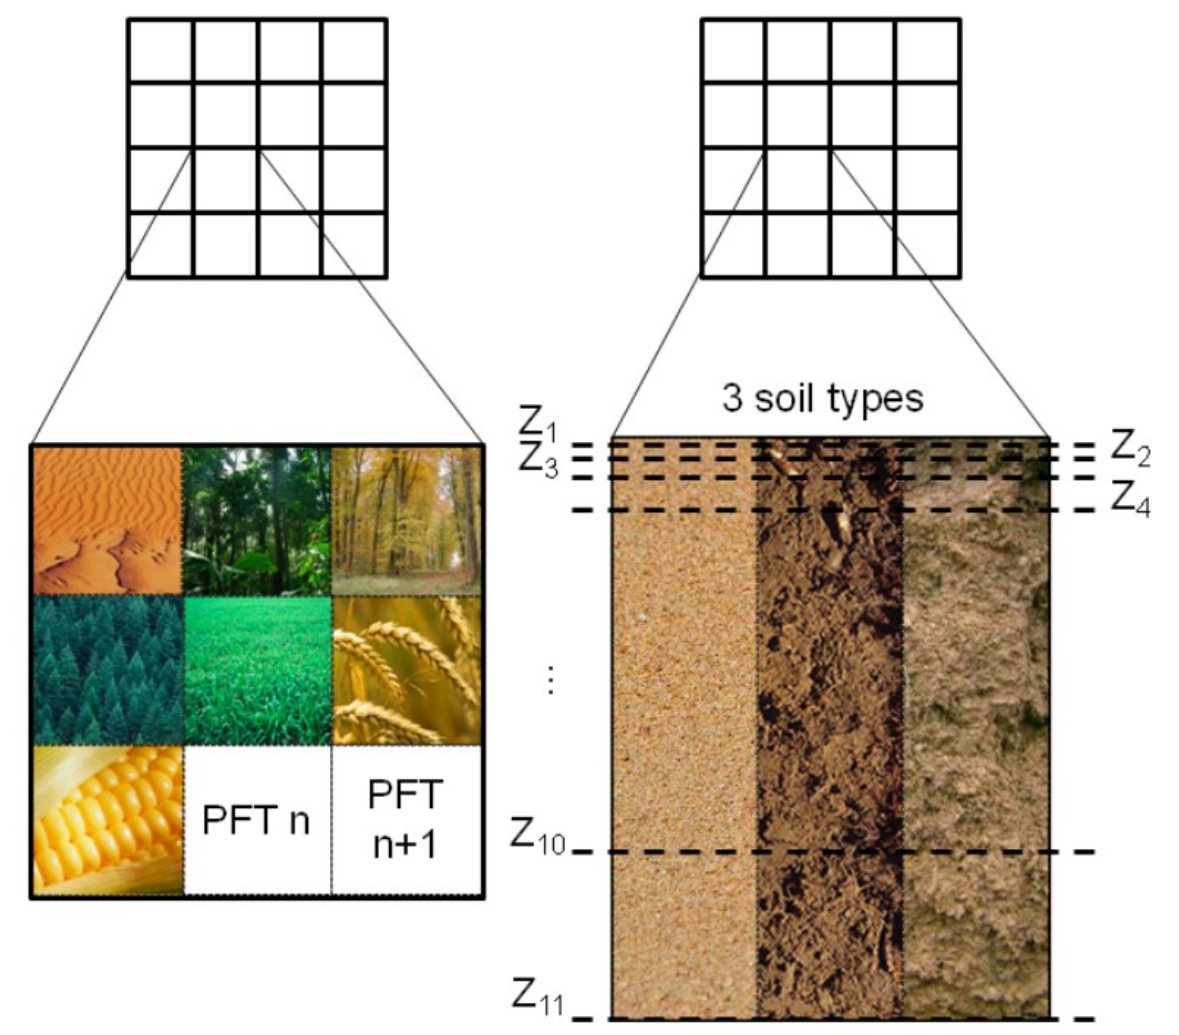
\includegraphics[width=0.5\textwidth]{images/methods/ORC_discretization.png}
    \caption{Visualisation of the ORCHIDEE PFTs and vertical discretization within one grid cell, (\href{https://orchidee.ipsl.fr/introduction/}{ORCHIDEE online documentation}).}
    \label{fig:ORC_discretization}
\end{figure}

\subsection{Water and energy budgets}\label{sec:water}

This section describes how the different terms of the water and energy budgets identified in the introduction are computed by ORCHIDEE, within the SECHIBA module. 

\subsubsection*{Precipitation partitioning}

To determine the soil water content in each soil tile of a grid cell, ORCHIDEE first separates the fraction of precipitation intercepted by vegetation and the fraction that actually reaches the ground. 
For liquid water that reaches the surface (either from rain or melted snow), it further discriminates between the portion that infiltrates into the soil and surface runoff, which occurs when infiltration is limited by hydraulic conductivity. Soil hydrology fluxes are based on the one-dimensional Richards equation, with a 2-meter soil column discretized over 11 vertical layers of increasing thickness \citep{de_rosnay_impact_2002, dorgeval_sensitivity_2008}, as shown in Fig. \ref{fig:ORC_discretization}. A free drainage condition is applied at the bottom of the column. ORCHIDEE models the infiltration front velocity, which progressively saturates the layers. The values of hydraulic conductivity and diffusivity are computed based on soil texture according to \citet{mualem_new_1976, van_genuchten_closed-form_1980}. As shown in Fig. \ref{fig:water_balance_AD}, the surface runoff and drainage computed in each grid cell then serve as input to the routing scheme, later described in Section \ref{section:routing_methods}.

Snow is represented with three layers of varying density and thermal conductivity \citep{wang_evaluation_2013}. The energy budget of the snowpack is computed, and when a layer's simulated temperature exceeds freezing, it is automatically reset to 0°C in the snow, and the excess energy is used to melt snow. The resulting liquid water may then percolate through the snowpack or be refrozen. If it reaches the soil surface, it is integrated into the surface water budget, contributing to infiltration and runoff in the same manner as rainwater.

\begin{figure}[hbtp]
    \centering
    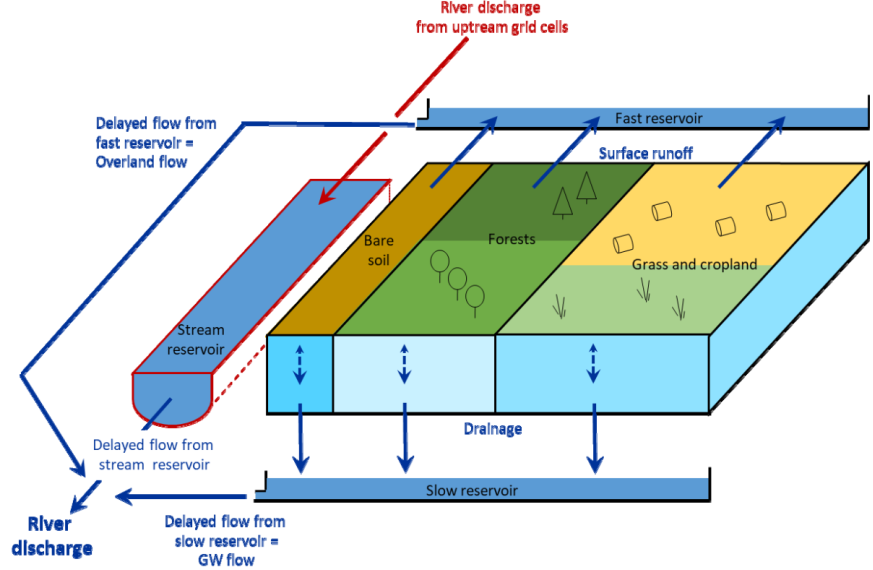
\includegraphics[width=0.8\textwidth]{images/methods/water_balance_AD.png}
    \caption{Visualisation of surface hydrology within an ORCHIDEE grid cell. (source: A. Ducharne, \href{https://forge.ipsl.fr/orchidee/attachment/wiki/GroupActivities/Training/cours_orchidee_feb2024_ducharne.pdf}{ORCHIDEE training}).}
    \label{fig:water_balance_AD}
\end{figure}


\subsubsection*{Potential and actual evapotranspiration}

The missing term to close the surface water balance is evapotranspiration $E$, which also appears in the energy balance via the latent heat flux $\lambda E$. The total evaporation value depends on potential evaporation, which represents the evaporation that would occur without water stress and thus serves as an upper limit. It is calculated using the formulation of \citet{Budyko_1956}:  

\begin{equation}
    E_{pot} = \rho_{air}  \lVert \vec{V} \rVert C_{drag, m} (q_{sat}(T_S) - q_{air})
\end{equation}

where $\rho_{air}$ is the air density, $\lVert \vec{V} \rVert$ is the horizontal wind speed, $C_{drag, m}$ is the surface drag coefficient for momentum (detailed description below), $q_{air}$ is the specific humidity of the air and $q_{sat}(T_S)$ is the specific humidity of saturated air at the surface temperature $T_S$. Air temperature, humidity, and wind speed are taken at the first level of the atmospheric model in coupled simulations, or at the height of the atmospheric forcing in offline simulations.

To obtain the actual evapotranspiration $E$ from the maximum theoretical value $E_{pot}$, ORCHIDEE computes the ratio of actual evapotranspiration to potential evapotranspiration $\beta = \frac{E}{E_{pot}}$, accounting for the four components of evapotranspiration:  

\begin{itemize}
    \item Bare soil evaporation, which is limited by the maximum volume that can be extracted from the soil column by upward water diffusion across one time step.
    %which is the minimum between $E_{pot}^*$, the potential evaporation reduced according to \citet{milly_potential_1992} and $Q_{up}$, the maximum volume that can be extracted from the soil column.
    %option:Tu peux preciser pourquoi on a besoin de Milly - Le sol n est pas une surface d'eau. Comment on evalue Q\_up - peut etre trop detaillé? 
    \item Vegetation transpiration, which is limited by the stomatal resistance of vegetation and a so-called architectural resistance which depends on vegetation structure.
    \item Evaporation of water intercepted by vegetation, which is also limited by the architectural resistance.
    \item Snow sublimation, which only concerns the regions and seasons where snowfall occurs.
\end{itemize}

To take into account these various limitations and the aerodynamic resistance which affects these four components of ET ($\frac{1}{\lVert \vec{V} \rVert C_{drag, m}}$), a conductance is identified for each component, and $\beta$ is computed as an effective conductance taking into account the fractions of the grid cell occupied by bare soil, vegetation and snow:

\begin{equation}
    \beta = f_{bare} \times \beta_{bare} + f_{veget} \times ( \beta_{transpiration} + \beta_{interception} ) + f_{snow} \times  \beta_{sublimation}
\end{equation}

It is important to note that although soil moisture might be different in each soil tile, $T_s$ (surface temperature), $C_{drag}$, and $\beta$ are computed for the whole grid cell. This means that there is a single $E_{pot}$ and evapotranspiration value for the grid cell, and therefore a single latent heat flux value.
This approach is often referred to as a composite approach, as opposed to a mosaic approach where independent fluxes are computed for each soil tile, before averaging them for coupling to the atmospheric model. 
%option: more details, limitations when comparing to obs (not able to obtain LE for a specific soiltile or PFT...), reference to Alice ?

% Bare soil evaporation is expressed as a relationship between supply and demand:
% \begin{equation}
%     E_g = min(E^*_{pot}, Q_{up})
% \end{equation}
% where $Q_{up}$ is the maximum volume that can be extracted from the soil column, and $E^*_{pot}$ is the reduced potential evaporation from \citet{Milly_1992}. Note that in most cases, $E^*_{pot} < E_{pot}$.
%NB Provide more details on the calculation of Qup? The available water volume is estimated by integrating Richards' equation over the soil column to maintain a water volume in each layer above......

% \hfill

% An alternative version exists in ORCHIDEE, which allows limiting the demand by modelling a bare soil resistance to evaporation $r_{soil}$ based on \citet{Sellers_1992}:
% \begin{equation}
%     E_g = min(\frac{E^*_{pot}}{1+\frac{r_{soil}}{r_a}}, Q_{up})
% \end{equation}
% \begin{equation}
%     r_{soil} = exp(8.206 - 4.255 \frac{W_L}{W_L^s})
% \end{equation}
% where $W_L$ is the moisture content in the top four layers of the soil column, and $W_L^s$ is the saturation moisture content in these same layers.

\hfill

\subsubsection*{Drag coefficients and roughness lengths}

There are two surface drag coefficients in ORCHIDEE, $C_{drag, m}$ for momentum and water vapour transfers, and $C_{drag, h}$ for heat transfers.
They can be computed for every PFT and depend on two roughness lengths: $z_{0m}$, below which wind speed is assumed to be zero, and $z_{0h}$, below which air temperature is assumed to be equal to the surface soil temperature. 
The default parametrization of roughness lengths in ORCHIDEE 2.2, used in this thesis, is based on \citet{su_evaluation_2001} and calculates them both dynamically, using empirical formulations which depend on the LAI. 
% However, some of the obtained values are not always consistent (particularly for $z_{0h}$), and another parametrization was introduced in ORCHIDEE, which will serve as default for CMIP7.
% With this simpler approach, the two roughness lengths depend on the canopy height of each PFT: 
% \begin{itemize}
%     \item The ratio between $z_{0m}$ and the canopy height, with a typical value of $\frac{z_{0m}}{h} = \frac{1}{15}$.
%     \item The ratio between $z_{0h}$ and $z_{0m}$, with a typical value of $\frac{z_{0h}}{z_{0m}} = \frac{1}{10}$.  
% \end{itemize}

Both drag coefficients car be expressed using a drag coefficient in neutral conditions and a stability function $f_H$:
\begin{align}
    &C_{drag,m} = C_{drag,m,neutral} f_H(Ri, z_{0m})\\
    &C_{drag,h} = C_{drag,h,neutral} f_H(Ri, z_{0m})
\end{align}

The coefficients for neutral conditions are calculated by taking into account the roughness lengths of all PFTs:
\begin{align}
    &C_{drag,m,neutral} = \sum_{i=1}^{N_\mathsf{PFT}} f_{veg,\max,i} \left[ \frac{k^2}{\left(\ln\left(\frac{z-d_{0,i}}{z_{0m,i}}\right)\right)^2} \right]\\
    &C_{drag,h,neutral} = \sum_{i=1}^{N_\mathsf{PFT}} f_{veg,\max,i} \left[ \frac{k^2}{\ln\left(\frac{z-d_{0,i}}{z_{0m,i}}\right)\ln\left(\frac{z-d_{0,i}}{z_{0h,i}}\right)} \right]
\end{align}
where ${d_{0,PFT}}$ is the displacement height, assumed equal to two thirds of the canopy height, ${k}$ is von Karman's constant and $z$ is the altitude of the atmospheric forcing.

The stability function depends on the Richardson number $Ri$, defined as the ratio of the two source terms for turbulent kinetic energy: buoyancy and wind shear, which depend on the gradient of temperature near the surface and on the surface wind speed. 
\begin{equation}
Ri= \frac{g}{\overline \theta} \frac{\frac{\partial \overline \theta}{\partial z}}{(\frac{\partial \overline u}{ \partial z})^2}
\end{equation}
A negative $Ri$ corresponds to an unstable atmosphere while positive values correspond to a stable one, and $Ri=0$ is the neutral case.
The stability function is defined differently for the unstable and stable cases, with two formulations from \citet{louis_short_1982}, which both converge towards $f_H(0)=1$.

\begin{equation}
f_H(Ri) = 
\begin{cases}
1 - \dfrac{3 B Ri}{1 + 3 B C C_{d,m,neutral} \sqrt{|Ri| \dfrac{z}{z_{0m}}}} & \text{if } Ri < 0 \\
\\
1 & \text{if } Ri=0\\
\dfrac{1}{1 + 3 B Ri \sqrt{1 + D |Ri|}} & \text{if } Ri > 0
\end{cases}
\end{equation}
with $B=C=D=5$.

\hfill

It must be noted that when ORCHIDEE is used in coupled mode with the atmospheric component of the IPSL-CM, LMDZ, ORCHIDEE does not fully compute the drag coefficients.
Instead, it computes only the neutral coefficients and provides LMDZ with effective roughness lengths for the grid cell $z_{0m,eff}$ and $z_{0h,eff}$. This modelling choice derives from the composite approach mentioned above, which is based on \textit{parameter aggregation}. Other land surface models use a mosaic approach, based on\textit{flux aggregation}, and compute turbulent fluxes for each PFT before averaging them to represent the grid cell.
Effective roughness lengths can be expressed as:
\begin{equation}
    z_{0m,eff}=z \exp{\left(\frac{-k}{\sqrt{C_{drag,m,neutral}}}\right)}
     \text{ and } 
    z_{0h,eff}=z \exp{\left(\frac{-k}{\sqrt{C_{drag,h,neutral}}}\right)}
\end{equation}
LMDZ then computes the drag coefficients using values from the surface layer for the Richardson number and its own stability functions. The formulation is similar for unstable cases, but for stable cases, functions from \cite{king_sensitivity_2001} are used:

\begin{equation}
f_{H, LMDZ}(Ri) = 
\begin{cases}
1 - \dfrac{3 B Ri}{1 + 3 B C C_{d,h,neutral} \sqrt{|Ri| \dfrac{z}{z_{0m}}}} & \text{if } Ri < 0 \\
1 & \text{if } Ri=0\\
(1-Ri/C_2)^2 & \text{if } 0 < Ri < C_2/2\\
(C_3(C_2/Ri)^2 & \text{if } Ri \geq C_2/2\\
\end{cases}
\end{equation}
with $B=C=5$, $C_2 = 0.25$, $C_3 = 0.0625$.

\hfill

\subsubsection*{Energy fluxes}
\label{sec:energy}
ORCHIDEE does not modify the incoming radiation terms but determines the outgoing reflected radiation terms by calculating the albedo (with distinct values for infrared and for visible light).

The heat flux into the ground, surface temperature (which controls the outgoing longwave radiation) and turbulent fluxes are computed with an implicit scheme which accounts for thermal diffusion in an 90-meter soil column discretized into 18 layers, with a zero-flux condition at the bottom. 
The vertical discretization matches the one used for water infiltration in the first two meters, and thermal conductivity and heat capacity are parametrized as a function of soil moisture and texture \citep{wang_improvement_2016}.
When coupled to LMDZ, semi-implicit coupling scheme is used to calculate the vertical transfer of heat by turbulent diffusion in the atmospheric column at the same time as thermal diffusion in the soil \citep{polcher_proposal_1998, Hourdin_phdthesis, hourdin_parameterization_2002, dufresne2009description}.
 It uses zero-flux boundary conditions at the top of the atmosphere and at the bottom of the 90-meter soil column, assuming no energy is transferred to the system at these interfaces.

The latent heat flux is expressed directly from the evapotranspiration detailed above:
\begin{equation}
    LE = \lambda \beta E_{pot} = \lambda \beta \rho_{air} \lVert \vec{V} \rVert C_{drag, m} (q_{sat}(T_S) - q_{air}),
\end{equation}
and the sensible heat flux:
\begin{equation}
    H = \rho_{air}  \lVert \vec{V} \rVert C_p C_{drag, h} (T_{s} - T_{air})
\end{equation}
where $\rho_{air}$ is the air density, $\lVert \vec{V} \rVert$ is the horizontal wind speed, $C_p$ is the is the specific heat of air, $C_{drag, h}$ is the surface drag coefficient for heat, $T_{air}$ is the air temperature, and $T_{s}$ is the surface temperature (sometimes referred to as the skin temperature).

\subsection{Routing scheme}
\label{section:routing_methods}
The routing scheme is a sub-module of SECHIBA, which simulates horizontal water transfers between grid cells and transports water to the oceans \citep{ducharne_development_2003, ngo-duc_validation_2007}. 
Water routing is necessary to maintain water conservation on a global scale in fully coupled simulations with a dynamic ocean model, and it also enables simulation of river discharge and groundwater volumes. 
This scheme generally runs at a larger time step than the rest of the model (once per day by default in global simulations). However, the irrigation scheme (Section \ref{sec:irrig_methods}) requires the routing to be performed at the same time step as the soil hydrology computed by SECHIBA. 

The routing scheme subdivides the simulation domain into hydrological transfer units (HTU) and uses a digital elevation model (DEM) constructed from topographic data to define flow directions and characterize the HTUs (dimensions, slope, upstream/downstream relationships). The grid of the HTUs, upon which the routing flows are solved, is often different from the ORCHIDEE grid, and is hereafter referred to as the routing grid.

Within each HTU, three linear reservoirs are represented: the \textit{slow} reservoir (groundwater), the \textit{fast} reservoir (overland water), and the \textit{stream} reservoir (rivers). For each reservoir, the characteristic residence time of water in one HTU depends on a fixed transfer coefficient (denoted TCST\_SLOW, TCST\_FAST, and TCST\_STREAM in Fig. \ref{fig:routing_principles}), on the size of the HTU and on the local slope obtained from the DEM.
Surface runoff and drainage computed for each ORCHIDEE soil column are regridded to the routing grid to respectively feed the overland and groundwater reservoirs. All three reservoirs then flow into the river reservoir of the downstream HTU. The river reservoir is therefore the only one connected to neighbouring HTUs, as no other horizontal transfer is modelled in ORCHIDEE. This assumption may have limitations at high resolutions as it ignores direct groundwater transfers between HTUs.

The outgoing water quantity $Q$ (given in $kg$) from a reservoir over one routing time step is expressed using the reservoir volume in the routing grid cell $V$ ($kg$), the transfer coefficient of the reservoir $TCST$ ($day \cdot km^{-1}$), a topographic index $topoindex$ ($km$), and the routing time step $dt_{routing}$ ($s$):

\begin{equation}
    Q = \frac{V}{topoindex \times TCST} \times \frac{dt_{routing}}{86400}
\end{equation}

The transfer coefficient reflects the roughness that creates a resistance to flow in this reservoir. The model assumes this parameter to be unique over the whole simulation domain, with a smaller value for the river reservoir than for the overland reservoir, and a larger one for the groundwater reservoir.
For a given DEM grid cell, the topographic index is defined as the length of the grid cell in the flow direction ($d$) divided by the square root of the slope, obtained from the altitude change $\delta z$ and $d$:

\begin{equation}
    topoindex = \frac{d}{\sqrt{\frac{\delta z}{d}}} = \sqrt{ \frac{d^3}{\delta z} } 
\end{equation}

\hfill

Several versions of the routing scheme have been developed in ORCHIDEE, all based on these modelling principles but corresponding to different relationships between the routing grid and the ORCHIDEE grid:

\begin{itemize}
\item \textbf{\textit{Subgrid\_halfdeg} routing}, which was the default option in branch 2.2 until CMIP6. It is designed to work with a specific DEM at a resolution of 0.5°.
Depending on the resolution of the ORCHIDEE grid, a given (whole) number of HTUs are defined within each ORCHIDEE grid cell. Since there are a whole number of HTUs in each ORCHIDEE grid cell, the regridding of surface runoff and drainage to the routing grid is only a partitioning using the areal fraction covered by each HTU.
Based on the DEM, a $topoindex$ value and slope direction are defined for each HTU using preprocessing scripts before starting the simulation.
In this manuscript, this routing was only used in Chapter \ref{chap:routing},  with an ORCHIDEE grid at 0.5° resolution, similar to the DEM, meaning there is always only one HTU per ORCHIDEE grid cell. 
It must be noted that this routing code is not compatible with non-regular ORCHIDEE grid cells, and can therefore not be used with the icosahedral grid of ICOLMDZOR.

\item \textbf{\textit{Subgrid\_HTU} routing}, largely based on \std, but adapted to used higher resolution DEMs \citep{nguyen-quang_orchidee-routing_2018, polcher_hydrological_2023}. However, this routing  also presents the constraint of having an integer number of HTUs within each ORCHIDEE grid cell, making it incompatible with the icosahedral grid of ICOLMDZOR. It was not used in the simulations presented in this thesis, but the manuscript occasionally refers to it.

\item \textbf{\textit{Interp\_topo} routing}, recently implemented by Yann Meurdesoif in ORCHIDEE to become the default version in IPSL-CM7. 
It is designed to adapt to any DEM resolution and to be completely independent of ORCHIDEE’s resolution and even of the shape of the grid cells. This is particularly necessary for compatibility with the icosahedral grid of the new atmospheric dynamics (DYNAMICO) of IPSL-CM7.
In this version, the routing grid is exactly the same as the DEM grid, meaning that the HTUs are exactly the DEM grid cells. This scheme relies on a robust interpolation \citep{kritsikis_conservative_2017} of runoff and drainage from the ORCHIDEE grid to the routing grid, where horizontal transfers between reservoirs are performed. Once these transfers are completed, water volumes in the reservoirs are re-interpolated from the routing grid back to the ORCHIDEE grid, allowing them to be used for irrigation within ORCHIDEE grid cells. 
A simplified calibration experiment had been carried out over the Danube basin \citep{kilic_evaluation_2023} but this PhD thesis provides the first evaluation and use case of this new routing in both offline and coupled simulations (Chapters \ref{chap:routing} and \ref{chap:monthly}).
Its principles are presented in Fig.\ref{fig:routing_principles}.
\end{itemize}


\begin{figure}[ht]
    \centering
    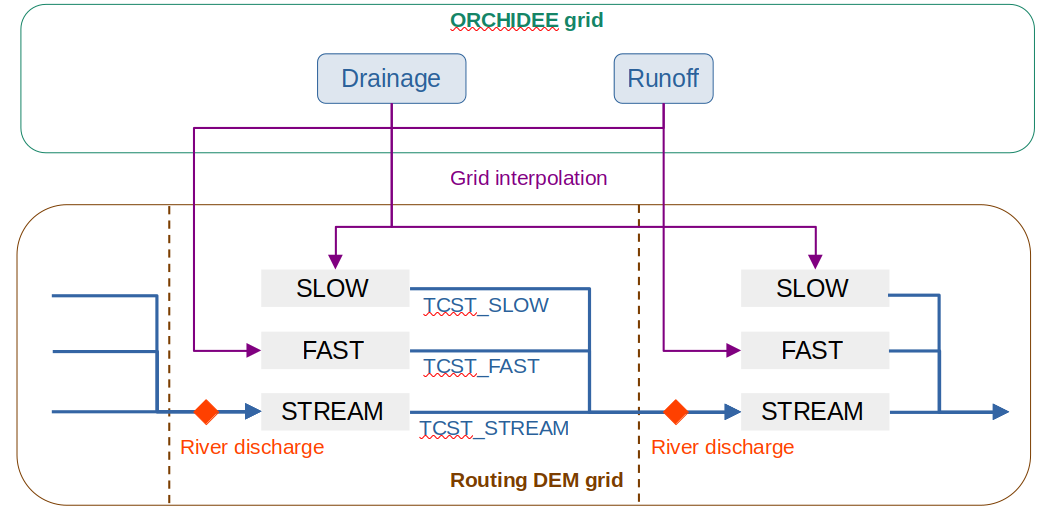
\includegraphics[width=1\textwidth]{images/methods/routing_principles.png}
    \caption{Modelling principles of the \textit{interp\_topo} routing.}
    \label{fig:routing_principles}
\end{figure}

Two DEMs are used in this work, with different resolutions. 
The first one is the 0.5° resolution DEM that has long been used within ORCHIDEE with the \std routing, based on the topography and flow directions of \citet{vorosmarty_geomorphometric_2000}.
The second one is a 1-arcminute ($\approx$ 2 km) resolution DEM based on the MERIT Hydro DEM \citep{yamazaki_merit_2019}.
The \std routing can only use the 0.5° DEM whereas the \native can be used with any DEM.

%option:show map of DEMs over the region -> not easy because big files on JZ but doable ?
%option:mention river discharge stations, positionning on DEM ? Or keep that for dedicated chapter ?

\subsection{Irrigation scheme}
\label{sec:irrig_methods}
\subsubsection{Modelling principles}

Irrigation has long been described in ORCHIDEE, using potential evapotranspiration as a target to define the irrigation amounts \citep{de_rosnay_integrated_2003, guimberteau_global_2012}. A new irrigation scheme was recently implemented in ORCHIDEE, presented and validated in \citet{arboleda-obando_validation_2024}. It is based on a water-conservative supply-and-demand approach, and uses a target soil moisture, more easily comparable with real irrigation practices, with more complex water allocation rules than the previous scheme. The present work relies solely on the new modelling approach, summarized in Figure \ref{fig:schema_pedro}.

\begin{figure}[t]
    \centering
    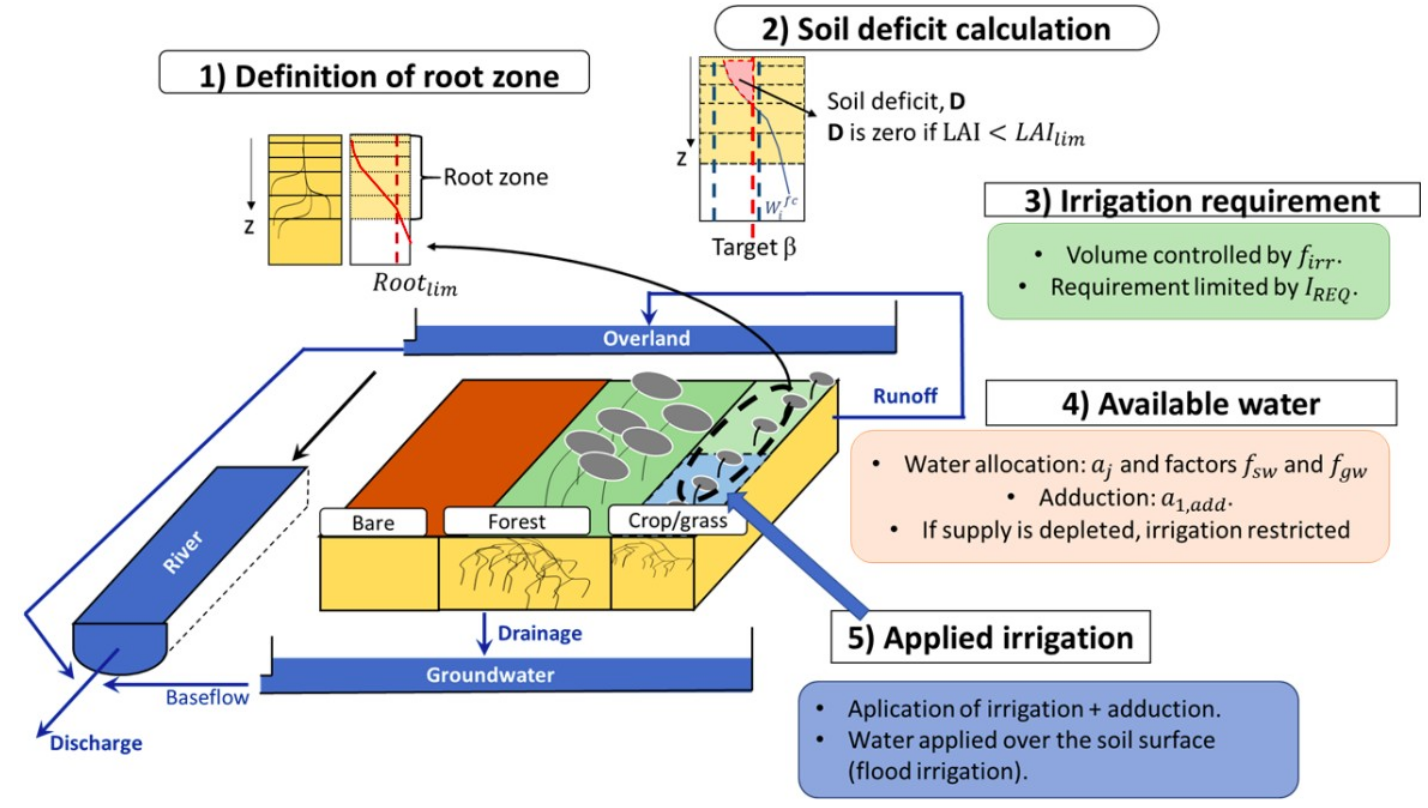
\includegraphics[width=1\textwidth]{images/methods/schema_pedro.png}
    \caption{Principles of the new irrigation scheme \citep[from][]{arboleda-obando_validation_2024}. Here, target parameter \betairrig is simply denoted $\beta$.}
    \label{fig:schema_pedro}
\end{figure}

First, an irrigated root zone is defined using parameter $z_{IRZ}$ in meters, which determines the depth of the considered root zone. In all the simulations presented here, $z_{IRZ} = 0.64$ was used, accounting for a 64-centimetre root zone. This value was selected in \citet{arboleda-obando_validation_2024} to account for 90\% of the root density in global simulations, and defined as the default parameter value. It is important to note that irrigation only applies to the column of low vegetation PFTs (grasses and crops), and the irrigated root zone is defined exclusively within this column.
A target soil moisture value is also defined, supposed to be optimal to sustain plant growth. It is expressed as a fraction of the soil moisture at field capacity water content (parameter \betairrig).

Given this target value and the soil moisture in the root zone, a soil moisture deficit $D$ (mm) is calculated as the sum of deficits across all layers of the root zone:
\begin{equation}
    D = \sum_{z_i < z_{IRZ}} min(0,\beta_{irrig} \times W_i^{fc} - W_i)
\end{equation}
where $W_i$ and $W_i^{fc}$ are respectively the soil moisture and field capacity soil moisture of layer $i$ (in mm).

In the absence of active vegetation (notably in winter), it is not relevant to compute a soil moisture deficit and an irrigation demand. A parameter $LAI_{lim}$ is therefore defined as a threshold LAI value below which the soil moisture deficit is zero. The default value is $LAI_{lim}=0.1$.

For a SECHIBA module time step $dt$ (by default 15 minutes in ICOLMDZOR simulations, 30 minutes in offline ORCHIDEE simulations), the irrigation demand hourly rate is $D/dt$ (mm/h). However, if the hourly irrigation rate is significantly higher than the infiltration rate into the soil, the model may produce excessive runoff that is not representative of reality. To prevent this, even if the moisture deficit is very high, the irrigation demand hourly rate is capped by a maximum value $I_{\max} = 3 mm \cdot h^{-1}$.

Finally, the water demand for the column is weighted by the fraction of the grid cell that is irrigated: $f_{irr}$. This fraction is obtained from the HID map at 5 arc-min resolution \citep{siebert_quantifying_2010}, and can be updated each year over the course of the simulation.
This irrigated fraction must not exceed the fraction of the soil column containing grasses and crops, as irrigation is only applied to this column.

The irrigation demand $I_{req}$ is therefore:
\begin{equation}
    I_{req} = f_{irr} \, \min(D/dt, I_{\max}).
\end{equation}

Once this demand is computed, the irrigation scheme searches for available water in the three routing reservoirs of the grid cell.
The volume of water available for irrigation is expressed as:
\begin{equation}
    A_w = f_{sw} \, (a_1 S_1 + a_2 S_2)+ f_{gw} \, a_3 S_3,
\end{equation}
where $S_i$ represents the water volume (in mm) in each of the reservoirs (rivers, overland, groundwater), and for each reservoir, a parameter $a_i \in [0;1]$ limits the total volume that can be withdrawn. This ensures that a certain amount of water remains in each reservoir, representing physical constraints and environmental regulations on irrigation withdrawals.
The fractions $f_{sw}$ and $f_{gw}$, ranging from 0 to 1, represent the accessibility of different reservoirs (surface water and groundwater, respectively) within the grid cell. These fractions are obtained from the global map of areas equipped for irrigation, from \citet{siebert_groundwater_2010}. A key feature of this map is that a given pumping point cannot be equipped for both surface water and groundwater use simultaneously, which translates to $f_{sw} + f_{gw} =1$.

Once the demand $I_{req}$ and supply $A_w$ are calculated, the applied irrigation is simply  determined as:
\begin{equation}
    I = \min(A_w/dt, I_{req}).
\end{equation}

Within the limit of $f_{sw}$ and $f_{gw}$, water is primarily withdrawn from the river reservoir, and only if this is insufficient to meet the demand are the other reservoirs tapped.
At the next time step, the amount of water withdrawn from the reservoirs, $I$, is added at the top of the ORCHIDEE soil column and infiltrates, simulating a gravity-fed or drip irrigation method.
It must be noted that although the original irrigation scheme from \citet{arboleda-obando_validation_2024} included the possibility to withdraw water from neighboring grid cells to represent adduction systems, this option is not yet compatible with the new version of the routing scheme used with ICOLMDZOR and was therefore not used in this work.

To summarize, Table \ref{tab:irrigation_parameters} gives the default value of all the parameters used by the irrigation scheme, while Fig. \ref{fig:irrig_inputs} shows the two input maps over the Iberian Peninsula: the map of irrigated fractions, to obtain $f_{irr}$, and the map of areas equipped for irrigation, to obtain $f_{sw}$ and $f_{gw}$. On Fig. \ref{fig:irrig_inputs}a, three main irrigated basins can already be noticed : the Ebro river basin in the Northeast, and the Guadiana and Guadalquivir basins in the South of the Peninsula. Differences can already be noticed between the Ebro, which has a large dependency on surface withdrawals, and the other two, which depend much more on groundwater withdrawals for irrigation (Fig. \ref{fig:irrig_inputs}b). This reflects different methods since in the Ebro valley water is mainly adducted from the Pyrenees, wheareas goundwater pumping is much more common and important in southern Spain.

The sensitivity analyses described in \citet{arboleda-obando_validation_2024} allowed the authors to define default values for all parameters to best match observed global irrigation when used uniformly, and showed that the target parameter \betairrig has the greatest impact on the volume of water withdrawn for irrigation.
In the default version of the global model, this parameter is set to 0.9, defining a soil moisture target at 90 \% of field capacity. However, this value reflects a wide variety of irrigation practices, from drip irrigation to flooding of rice paddies, and had to be adjusted for simulations over the Iberian Peninsula as discussed in Chapter \ref{chap:routing}.

\begin{table}[htbp]
    \centering
    \begin{tabular}{|l|p{7cm}|c|}
        \hline
        \textbf{Parameter name} & \textbf{Description} & \textbf{Default value} \\
        \hline
        $z_{IRZ}$ & Root zone depth. & 64 cm \\ %cum_dh_thr
        \hline
        \betairrig & Target soil moisture (as a percentage of soil moisture at field capacity). & 90 \% \\%beta_irrig
        \hline
        $LAI_{lim}$ & Minimum leaf area index (LAI) threshold for irrigation activation. & 0.1 \\ %lai_irrig_min
        \hline
        $I_{max}$ & Maximum allowable irrigation rate. & 3 mm $\cdot h^{-1}$ \\ %irrig_dosmax
        \hline
        $a_i$ & Fraction of reservoirs that can be withdrawn. & 90 \%  (for each reservoir)\\ %avail_reserv
        \hline
    \end{tabular}
    \caption{Parameters used in the irrigation scheme and their default values.}
    \label{tab:irrigation_parameters}
\end{table}

\begin{figure}[htbp]
    \centering
    \begin{subfigure}[b]{0.48\textwidth}
        \caption{}
        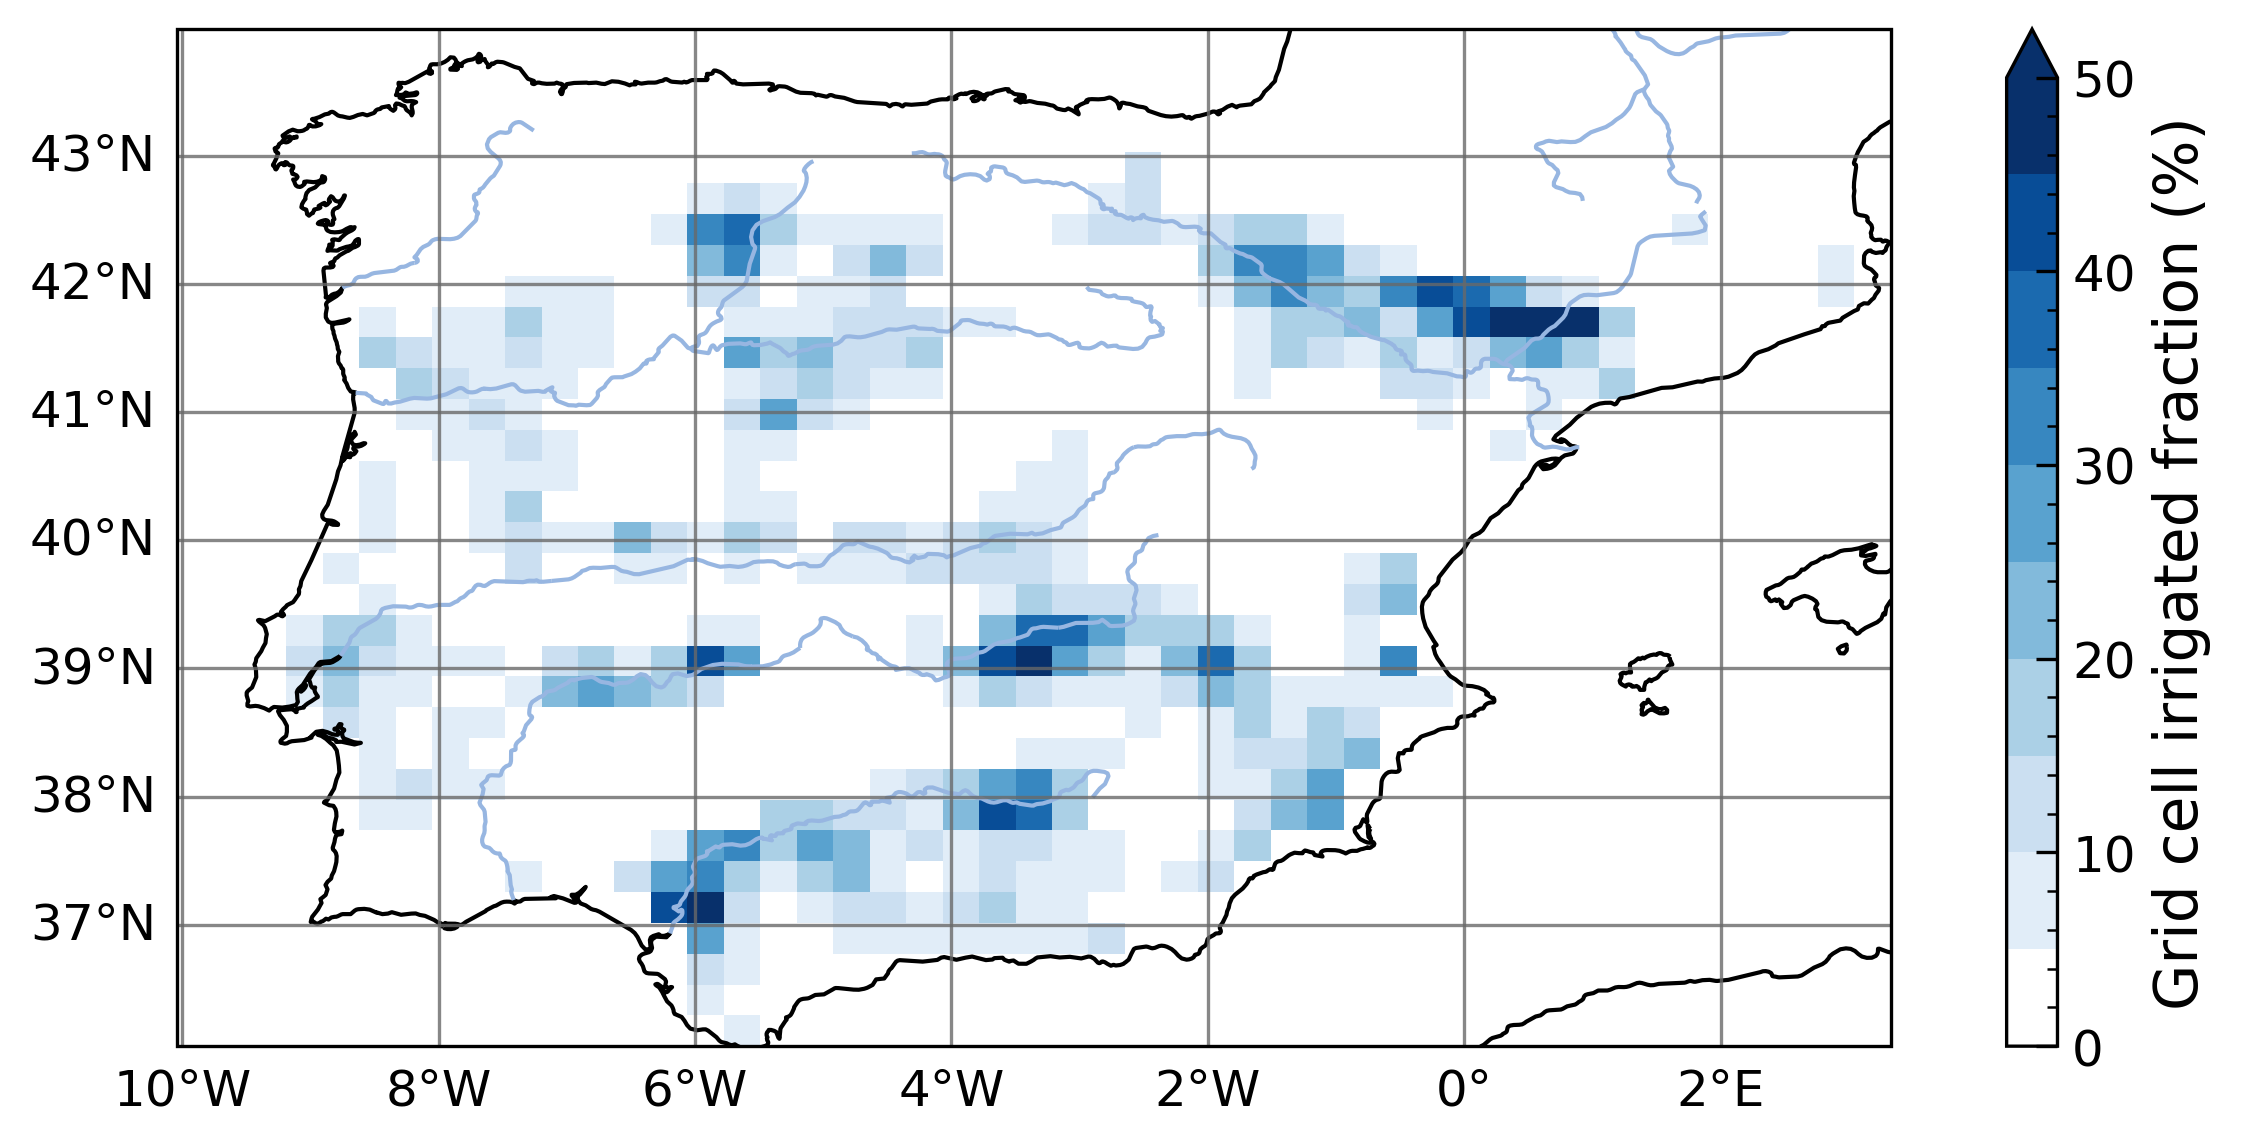
\includegraphics[width=\textwidth]{images/methods/irrigated_fraction_map.png}
    \end{subfigure}
    \begin{subfigure}[b]{0.48\textwidth}
        \caption{}
        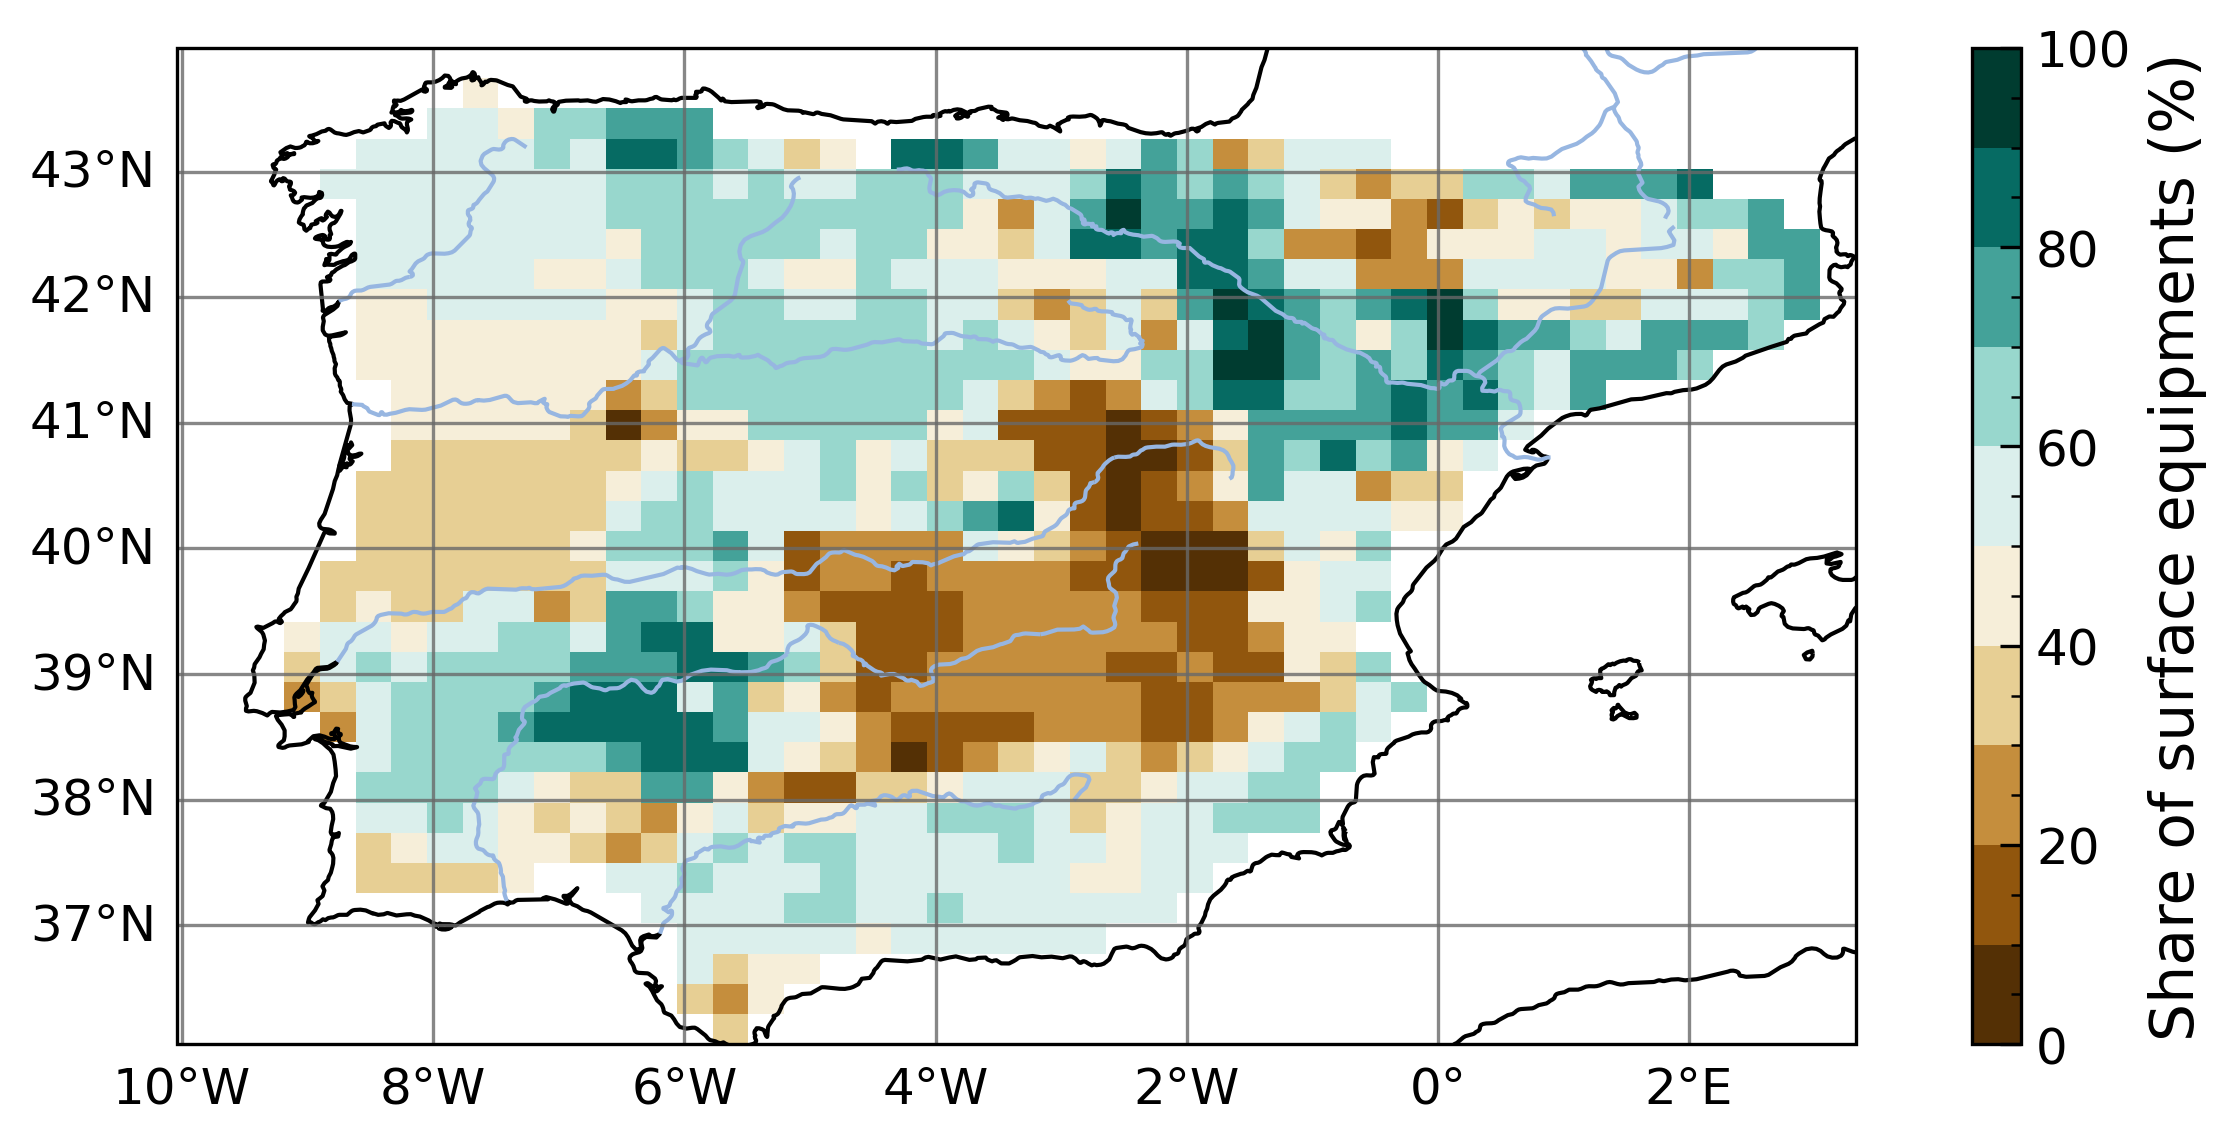
\includegraphics[width=\textwidth]{images/methods/aei_sw_map.png}
    \end{subfigure}
    \caption{Input maps of the irrigation scheme over the study area: (a) grid cell irrigated fraction \citep[\%, derived from][]{hurtt_harmonization_2020}, and (b) the share of surface equipments for irrigation withdrawals, as opposed to groundwater withdrawals \citep[\%, derived from][]{siebert_groundwater_2010}.}
    \label{fig:irrig_inputs}
\end{figure}

\subsubsection{Irrigation scheme with the \native routing.}
\label{sec:irrig_interp_variables}

This irrigation scheme was initially developed for the \std routing version, and adjustments were made when developing the \native routing to make it compatible with this new routing code. Since the routing grid is completely independent of the ORCHIDEE grid in \native, it is important to identify which variables are computed directly on the ORCHIDEE grid and which ones are computed on the routing grid, and then interpolated to the ORCHIDEE grid to be used as ORCHIDEE outputs.
In particular, reservoir volumes are computed on the routing grid, which means that irrigation (which withdraws from these reservoirs) must be computed on the same grid.
To ensure water conservation, the \native routing uses absolute values in $kg$ of water (as opposed to areal values in $kg \cdot m^{-2}$). Therefore, when interpolating variables from one grid to another, the variables are also converted to a different unit, accounting for the continental area of the ORCHIDEE grid cells.
The only variable that is output directly on the routing grid is the river discharge, which cannot be averaged in a conservative way. Since the routing grid is of higher resolution than the ORCHIDEE grid, it also enables a more relevant comparison to discharge observation stations.
Figure \ref{fig:irrig_interpolations_outputvars} summarizes the interactions between the two grids for routing and irrigation variables in \native.

\begin{figure}[htbp]
    \centering
    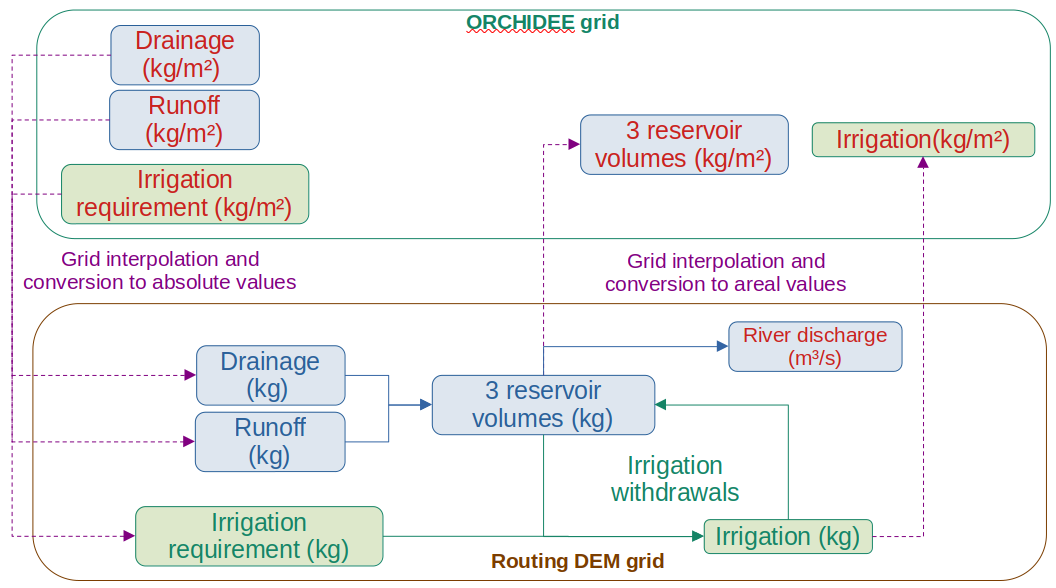
\includegraphics[width=\textwidth]{images/methods/routing_irrig_interpolation_outputvars.png}
    \caption{River routing and irrigation variables and interactions between the ORCHIDEE and routing grids in \native. Variables shown in red are used as model outputs while the others are only intermediate computations.}
    \label{fig:irrig_interpolations_outputvars}
\end{figure}

\section{Atmospheric model : the ICOLMDZ LAM}
\label{sec:ICOLMDZLAM}

In \atmchapters, coupled simulations are run with ORCHIDEE and atmospheric model ICOLMDZ in a limited area model (LAM) configuration, first used and described in \citet{raillard_leveraging_2024}. 
It must be noted that the use of the LAM in the IPSL community is very recent, and that its development and evaluation are still ongoing. In particular, the simulations presented in Chapter \ref{chap:monthly} constitute the first case study focusing on the water cycle and land-atmosphere interactions, as well as the first use case at the mid-latitudes.

\subsection{Dynamical core and parametrizations}
ICOLMDZ, the atmospheric component of the model is the association of the dynamical core DYNAMICO \citep{dubos_dynamico-10_2015}, and the LMDZ6A physics used for CMIP6 \citep{hourdin_lmdz6a_2020}. 
Icosahedral dynamical cores already existed in some models, such as ICON \citep{zangl_icon_2015,giorgetta_icon-_2018,prill_icon_2022}, and DYNAMICO was introduced in the IPSL-CM with the main objectives of unlocking a high level of parallelization and standardizing grid cells for global simulations. 
In particular, it avoids the discrepancies of a regular longitude-latitude grid that appear at the poles, opening new prospects for modelling projects in the Arctic \citep{raillard_leveraging_2024} and Antarctic regions \citep{wiener_extensive_2025}.
All ICOLMDZ simulations run in the thesis used a 30-second time step for the dynamics.

The physics of the model is version NPv6.2 with 79 vertical levels, and is run every 15 min, although some processes are not called at every time step to limit computation time.
The physics include the following parametrizations:
\begin{itemize}
    \item a surface layer description based on Monin-Obukhov similarity theory \citep{monin1954osnovnye}, using formulations from \cite{louis_parametric_1979} and \cite{king_sensitivity_2001}; 
    \item an Eddy-Diffusivity Mass Flux (EDMF) scheme of boundary layer vertical transfer composed of a turbulent diffusion scheme based on \cite{yamada_simulations_1983} with recent improvements described in \cite{vignon_modeling_2018}, and a thermal plume model for shallow convection \citep{rio_thermal_2008, hourdin_unified_2019}; 
    \item a mass-flux scheme for deep convection based on Emanuel's scheme \citep{emanuel_scheme_1991, grandpeix_improved_2004, rio_control_2013}, with stochastic triggering \citep{rochetin_deep_2014, rochetin_deep_2014-1}, called every 30 minutes; 
    \item a parametrization of the cold pools created below cumulonimbus by reevaporation of convective rainfall \citep{grandpeix_density_2010-1,grandpeix_density_2010};
    \item a large scale condensation scheme based on a statistical distribution of sub-grid total water content, from which cloud fraction and water contents are derived \citep{madeleine_improved_2020}; 
    \item the radiative transfer model RRTM \citep{mlawer_radiative_1997}, which is called every 1.5 hours (six time steps).
\end{itemize}

\subsection{Forcings}

All simulations were run with spectral solar irradiance from CMIP6 solar forcing \citep{matthes_solar_2017}, distinguishing between the historical period (until 2014) and future reference scenario (from 2015).
Greenhouse gases concentrations in the atmosphere were taken from the CMIP6 historical forcing dataset for CO2, CH4, N2O, as well as CFC 11 and 12.
Aerosols forcings were also taken from the forcing created for CMIP6 runs with the INCA module of the IPSL-CM \citep{hauglustaine_global_2014}, as detailed in \citet{lurton_implementation_2020}.
Considering that the simulations were rather short and that the focus was on the impact of irrigation, the greenhouse gases and aerosol values from 2014 were used for the period 2015-2022. For future climate simulations with a focus on climate change (Section \ref{sec:climate_change}), the values that follow the SSP5-8.5 were used.

The atmospheric model is not coupled with an ocean model and uses prescribed sea surface temperature (SST) and sea ice content (SIC). For recent climate simulations (2010-2022), monthly values at 1° resolution are taken from the PCMDI-AMIP-1.1.9 boundary conditions dataset, which is based reanalysis products \citep{taylor_sea_2000, hurrell_new_2008}.
%todo:future : voir avec Frédérique (SST corrigées, par qui et comment ?)

\hfill

Since simulations with the LAM only cover a portion of the globe, lateral boundary conditions (LBC) must be read by the model from a forcing file. They can be obtained from various sources of different type, spatial resolution, and sampling frequency. 
The influence of the LBC is a well known problem in regional climate modelling or dynamical downscaling. 
\citet{denis_sensitivity_2003} analysed the dependency of the simulated climate to the resolution of the LBC and found that a 12 times lower spatial resolution in the forcing compared to the domain could still yield acceptable performance. This study also explored the influence of the temporal sampling and little difference between a 3-hour and a 6-hour sampling, but a degradation of performance with a 12-hour sampling frequency.
\citet{wu_estimating_2005} performed regional climate model simulations with LBC obtained from 16 different sources and found them to be more impactful than the initial conditions, and that climate variables such as precipitation could be affected by the choice of forcing source over the whole simulation domain. 
The sensitivity of variables such as precipitation or sea level pressure to the LBC was found to be improved with larger simulation domains \citep{koltzow_importance_2011}, although \citet{leduc_sensitivity_2011} showed that this effect was very dependent on the local climate and even on the season.

In most of the work presented here, lateral boundary conditions for the LAM were taken from ERA5 reanalysis hourly values at 0.25° resolution \citep{hersbach_era5_2020}. This product uses a climate model with observation data assimilation techniques to produce outputs that are as close as possible to actual conditions. When simulating recent climate, using this forcing enables having rather realistic synoptic conditions. 
It is also possible to run the model with other sources for the forcing file, in particular using outputs from global climate simulations, either from the ICOLMDZOR global model or from other models. The modelling community at IPSL is also currently investigating the possibility of using outputs from the CMIP6 simulations under various SSPs to run the LAM in projected future climate conditions.
In this work, hourly forcing files were used for most of the simulations, but some sensitivity experiments were made using forcing data sampled every six hours, which is the sampling frequency of CMIP6 outputs. Section \ref{sec:sim_setups} details all the simulation setups used to produce the results presented in Chapters \ref{chap:forcing} and \ref{chap:monthly}.

To run a regional simulation, the forcing file must contain data for the nudged variables (temperature, humidity, wind), two variables describing clouds (liquid and ice water content) used on the edge of the domain but not nudged, and three other variables at the surface that are used to manage initialization (2-meter temperature, geopotential height), and vertical interpolation (surface pressure). In the future, the model developers are considering a simpler forcing file without the cloud liquid and ice water content, as it is not very standard to use such variables in regional modelling, and these variables are not available in CMIP standardised outputs. 

\begin{table}[htbp]
\centering
\begin{tabular}{|l|l|}
\hline
\multicolumn{2}{|c|}{\textbf{Variables nudged on vertical levels}} \\ \hline
Air temperature                & t     \\ \hline
Zonal wind                    & u     \\ \hline
Meridional wind               & v     \\ \hline
Relative humidity             & r     \\ \hline
Specific humidity             & q     \\ \hline
\multicolumn{2}{|c|}{\textbf{Cloud variables, on vertical levels}} \\ \hline
Specific liquid water content & clwc  \\ \hline
Specific ice water content    & ciwc  \\ \hline
\multicolumn{2}{|c|}{\textbf{Surface variables}} \\ \hline
2-meter air temperature            & t2m   \\ \hline
Surface geopotential          & z     \\ \hline
Surface pressure              & p     \\ \hline
\end{tabular}
\caption{List of lateral boundary conditions and surface variables required in the LAM forcing file.}
\end{table}

\subsection{LAM domain structure and nudging method}

The simulation domain is a large hexagon divided into hexagonal grid cells, and defined by three parameters:
\begin{itemize}
    \item The centre of the hexagon (latitude and longitude).
    \item The radius of hexagon, distance between the centre and one of the vertices, in kilometers.
    \item The number of grid cells on this radius, referred to as NBP.
\end{itemize}

The resolution of the model (diameter of one grid cell) is directly obtained by dividing the radius by the NBP.

\hfill

The simulation domain is separated in 3 concentric zones, as shown on Fig. \ref{fig:LAM_domain}: 
\begin{itemize}
    \item The "raw forcing zone" which contains values directly given by the forcing, consisting of 5 grid cells.
    \item The "transition zone"  where the model is nudged toward the forcing with decreasing strength, consisting of 8 grid cells.
    \item The "free zone" at the centre of the domain where there is no direct influence of the lateral forcing, with all the remaining grid cells (NBP - 8 - 5).
\end{itemize} 

\begin{figure}[ht]
    \centering
    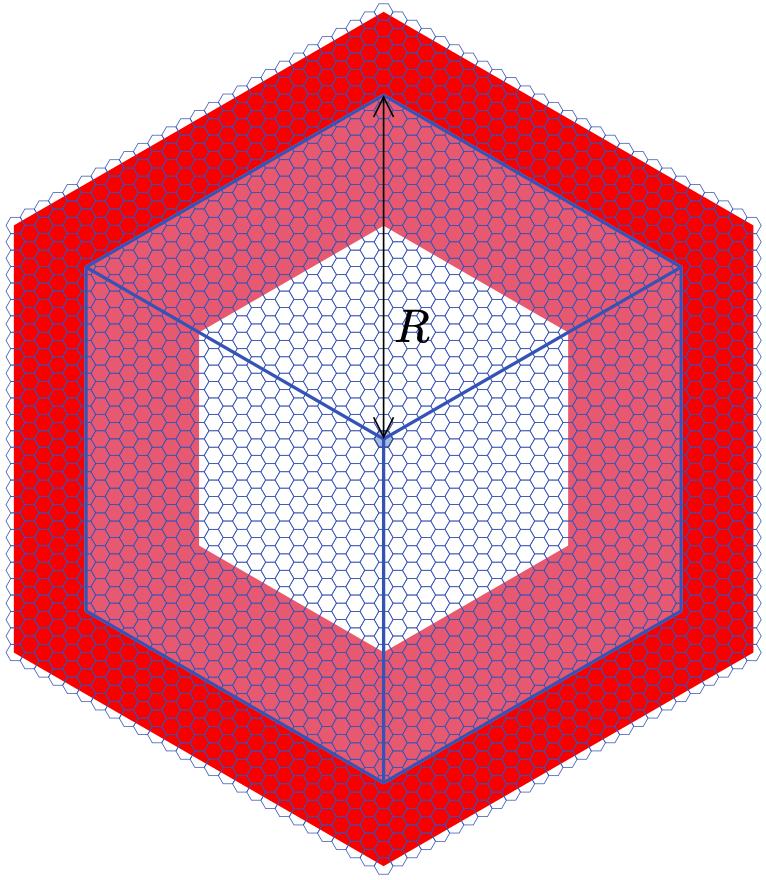
\includegraphics[width=0.5\textwidth]{images/methods/LAM_domain_zones.png}
    \caption{LAM domain structure example with NBP=27 \citep[from][]{raillard_leveraging_2024}}. The raw forcing zone is in red on the outside, the transition zone in pink, and the free zone in white at the center.
    \label{fig:LAM_domain}
\end{figure}

The concept of nudging is well known in climate modelling and NWP, since it is used to manage lateral boundary conditions in regional models. It is also used to reproduce real situations to enable the comparison to local observations with realistic synoptic conditions, or to study specific observed events with a model. 
Multiple studies were conducted using the zoom capability of LMDZ to enhance resolution over a given area, while nudging the model towards a reanalysis in the rest of the world to make sure the synoptic conditions are as close to reality as possible. In particular, land-atmosphere interactions were studied with zoomed-nudged LMDZOR simulations at the SIRTA observation site in France \citep{cheruy_combined_2013, campoy_response_2013} and over Morocco \citep{balhane_global_2022, arjdal_modeling_2024}. The main downside of this approach is that it still requires to run the model in a global simulation setup, although the grid is stretched to focus on the area of interest. With the LAM, the resolution remains the same in all the domain and the model is only run over the area of interest, which results in lower computation times than zoomed-nudged setups for a given resolution.
%todo:Ajouter commentaires et odg sur le temps de calcul, cf simus de Frédérique : global vs LAM, nombre de tasks donc d'heures de calcul. Avantages ou non par rapport au zoomé-guidé (qui peut être forcé par ERA) 

The model is nudged by adding a forcing term in the equation that governs the evolution of a given prognostic variable $V$ in the model, to drive it towards a reference value $V_{ref}$ over a given time scale $\tau$:

\begin{equation}
    \frac{\partial V}{\partial t} = \frac{\partial V}{\partial t}_{\text{model}}+ \frac{V_{\text{ref}} - V}{\tau}.
\end{equation}

The strength of the nudging can be modulated by adjusting the time scale $\tau$.
In the raw forcing zone, the values of the state variables in the model are directly prescribed to those of the lateral boundary conditions in the forcing file. 
In the central free zone, $\tau$ is infinite, meaning the forcing term does not alter the equation. 
In the transition zone, the value of $\tau$ is gradually increased over the 8 grid cells, following an arctan profile to smooth the transition, starting from $\tau = 3600$ s on the outer edge.
Nudging is applied on all vertical levels at every time step of the dynamics (30 s). The reference value for each variable is obtained by temporally interpolating the forcing file to this time step. 

\section{Coupled simulation setups}
\label{sec:sim_setups}
\subsection{Simulation domains, periods and forcing data}

Several simulation setups and periods were used to produce the results presented in \atmchapters, but they all used a hexagonal domain centered at (40.4°N, -3.7°E), with a radius ($R_{domain}$) of either 1000km, 1500km or 2000km. When changing the radius of the domain, the $NBP$ parameter (number of grid cells on the domain radius) was adapted to either 40, 60, or 80, to ensure that grid cells kept the same diameter of 25km. The setup with a $R_{domain}=1500 km$ and $NBP=60$ is presented in Fig. \ref{fig:domain_full_hex}. 
Since the spatial resolution was always the same, the timesteps were also fixed, to 30s for the dynamical core, and 15mn for the atmospheric physics and the LSM (including routing and irrigation). 

%figure:altitude over hexagonal domain (native grid)
\begin{figure}[hbtp]
    \centering
    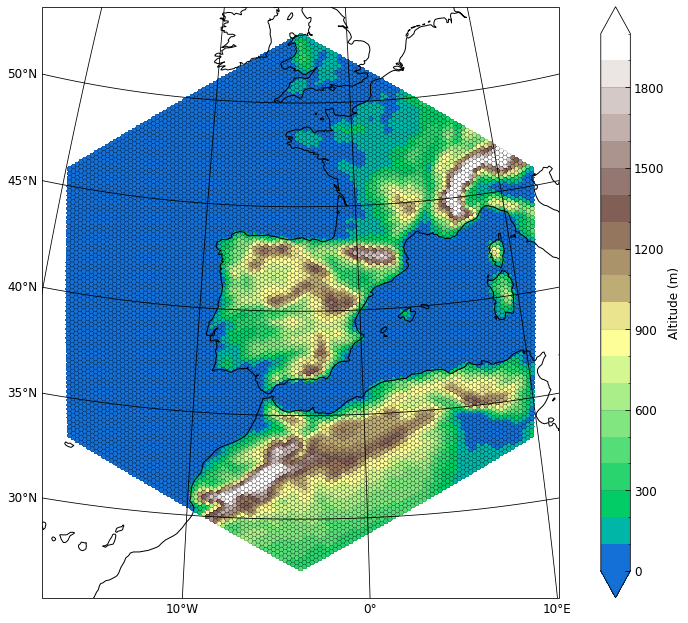
\includegraphics[width=0.7\textwidth]{images/chap4/article/f01.png}
    \caption{Altitude (m) over the simulation domain on the native hexagonal grid for a simulation with $R_{domain}=1500 km$ and $NBP=60$.}
    \label{fig:domain_full_hex}
\end{figure}


Forcing files from two different sources were used, and the differences this choice can induce are analysed in Chapter \ref{chap:forcing}. In Chapter \ref{chap:monthly}, the forcing variables are from the ERA5 reanalysis over the period 2010-2022 (Section \ref{sec:article1}), while for the study of climate change over the Iberian Peninsula (Section \ref{sec:climate_change}), outputs from a global ICOLMDZOR simulation under greenhouse gases emission scenario SSP5-8.5 were used as forcing variables.
Sensitivity tests on the impact of the forcing file sampling frequency are also presented in Chapter \ref{chap:forcing}, with forcing files containing either hourly or 6-hourly data.
This sensitivity was of interest since future climate simulations were initially supposed to use CMIP6 output variables, which are available only every six hours. However, this option was eventually discarded due to technical difficulties such as unexpected model crashes when running simulations with this sampling frequency and issues with the formatting of the forcing file from CMIP6 outputs. The future climate simulations presented in Chapter \ref{chap:monthly} were therefore run using hourly outputs from a global ICOLMDZOR simulation.

%option: for ICOLMDZOR forcing, detail zoom parameters

The main study period under current climate is from 2010 to 2022, since before and after that period not all forcing variables were readily available on the IPSL servers and running the LAM would have required substantial manual data collection work. Some sensitivity analysis of Chapter \ref{chap:forcing} were run on specific or shorter periods to overcome technical issues or to limit the computing time and ressources used.
All simulations were run after a 3-year spinup period to make sure that vegetation and hydrological variables had reached an equilibrium. 
To analyse the impact of domain size, simulations were only run between 2010 and 2014. 
For the analysis of the forcing file sampling frequency, simulations were only run over the year 2013 because of unexpected model crashes in other simulation years. This same year was run 10 times in chained simulations (starting each new simulation year at the end of the previous one) that can act as a small ensemble, although it must be noted that this secific year cannot represent the diversity of current climate by itself.
Simulations of future climate were run over the period 2050-2062, using hourly outputs from a global ICOLMDZOR simulation, and the smaller domain configuration. 

The characteristics of all the coupled simulation used in this thesis are summarized in Table \ref{table:coupled_simulations}.

%table:all coupled simulation details
\begin{table}[h]
    \centering
    \resizebox{\textwidth}{!}{
        \begin{tabular}{|l|l|l|l|l|l|l|l|}
            \hline
            \textbf{Section} & \textbf{Simulation name} & \textbf{Period} & \textbf{Diameter} & \textbf{NBP} & \textbf{Forcing (source, frequency)} & \textbf{Irrigation} \\
            \hline
            \ref{sec:domain_size} & \smalld & 2010-2014 & 1000km & 40 & ERA5, 1h & No \\
            \hline
            \ref{sec:domain_size}  & \interd & 2010-2014 & 1500km & 60 & ERA5, 1h & No \\
            \hline
            \ref{sec:domain_size}  & \larged & 2010-2014 & 2000km & 80 & ERA5, 1h & No \\
            \hline
            \ref{sec:forcing_source} & \forcingERA & 2010-2022 & 1000km & 40 & ERA5, 1h & No \\
            \hline
            \ref{sec:forcing_source} & \forcingICO & 2010-2022 & 1000km & 40 & ICOLMDZOR, 1h & No \\
            \hline
            \ref{sec:forcing_frequency} & \forcingoneh & 2013 (* 10) & 1500km & 60 & ERA5, 1h & No \\
            \hline
            \ref{sec:forcing_frequency} & \forcingsixh & 2013 (* 10) & 1500km & 60 & ERA5, 6h & No \\
            \hline
            \ref{sec:article1}, \ref{chap:liaise} & \irr & 2010-2022 & 1500km & 60 & ERA5, 1h & Yes \\
            \hline
            \ref{sec:article1}, \ref{chap:liaise} & \noirr & 2010-2022 & 1500km & 60 & ERA5, 1h & No \\
            \hline
            \ref{sec:climate_change} & \presnoirr & 2010-2022 & 1000km & 40 & ICOLMDZOR, 1h & No \\
            \hline
            \ref{sec:climate_change} & \futnoirr & 2050-2062 & 1000km & 40 & ICOLMDZOR, 1h & No \\
            \hline
            \ref{sec:climate_change} & \futirr & 2050-2062 & 1000km & 40 & ICOLMDZOR, 1h & Yes \\
            \hline
        \end{tabular}
    }
    \caption{Coupled simulations characteristics.}
    \label{table:coupled_simulations}
\end{table}

\subsection{Technical specificities}

While running the first simulations with the LAM, various occurrences of inappropriate model behaviour were observed at the top of the atmosphere, reaching temperatures over 373 K. Based on prior experience of the model developers, this was attributed to inconsistent quantities of air in these layers of very low density, which could lead to excessive heating over one model time step. The unusual interaction of advection from the dynamics and nudging were thought to be responsible for anomalies in the mass and energy budgets, in or near the transition zone.
To solve this issue, an additional nudging of temperature and wind components was applied for the upper layers of the atmosphere (above 1hPa) over the whole domain (including the free zone), to ensure that values remains in a reasonable order of magnitude. Given the focus on land-atmosphere interactions, this technical fix for the upper atmosphere is not considered to have any influence on the results.

It must also be noted that the model computes all variables on its hexagonal grid cells. However, analysing and displaying simulation data on such a grid is challenging because most standard tools (Ferret, ncview, Matplotlib) do not natively support its coordinate system. 
By default, LAM outputs are therefore interpolated to a more traditional longitude-latitude grid of similar resolution, to simplify posttreatment and comparisons to evaluation products, but can be obtained on the native hexagonal grid if needed.
The simulations used in Chapters \ref{chap:forcing} and \ref{chap:monthly} were analysed solely using the interpolated outputs, while simulations used in Chapter \ref{chap:liaise}, which focused on specific grid cells for comparison to observation, were analysed using outputs on the native hexagonal grid.

Considering the focus on land-atmosphere coupling, the analysis is often restricted to the Iberian Peninsula, thus excluding ocean grid cells and the land grid cells north of the Pyrenees, which flow to France. To prevent mismatches between the simulations and the evaluation datasets because of different coastlines, the analysis is further reduced to grid cells where the continental fraction is greater than 95\%. 

\section{Evaluation datasets}
\label{sec:eval_datasets}

The simulations in present climate conditions (Chapter \ref{chap:forcing}, Section \ref{sec:article1}) were evaluated against the monthly mean values of several reference gridded products listed in Table \ref{tab:obs-datasets}.
The ERA5 reanalysis \citep{hersbach_era5_2020} at 0.25° resolution was first used as a reference product to asses the realism of multiple variables (precipitation, ET, 2-m temperature), and this is how some inconsistencies studied in Chapter \ref{chap:forcing} were identified. However, in most simulations, ERA5 was the source used for the lateral boundary conditions which does not make it the most appropriate reference product for evaluation. Moreover, although ERA5 contains a lot of variables and has the advantage of being available over all the domain and present simulation period, some variables are more dependent on the model used to produce the reanalysis than on data assimilation and may not be the best reference for evaluation. Therefore, other reference products were also used, for precipitation and evapotranspiration.

Precipitation data from the Global Precipitation Climatology Centre (GPCC) Full Data Monthly Product Version 2020 \citep{gpcc_v2020} was used. This product provides precipitation data until 2019 over land on a 0.25° x 0.25° grid using in situ rain gauges. 

For ET, the Global Land Evaporation Amsterdam Model (GLEAM) dataset was used, in its fourth version \citep{miralles_gleam4_2025}. This product computes ET using a large set of input variables obtained from reanalyses as well as in situ and satellite observations. Monthly values at 0.25° resolution were used, initially given in mm month$^{-1}$ and converted to mm d$^{-1}$. GLEAM4 is available until 2022 but when precipitation and ET were evaluated jointly (Sections \ref{chap:forcing}, \ref{sec:article1}), it was only used over the availability period of GPCC data (2010-2019).

Simulated irrigation was evaluated in the Ebro Valley region using a high resolution remote sensing product from the European Space Agency (ESA) Irrigation+ project \citep{dari_regional_2023}. This product estimates irrigation with a soil moisture based approach using satellite measurements from Sentinel-1, and provides data for three intensely irrigated areas: the Ebro Basin in Spain, the Po Valley in Italy and the Murray-Darling Basin in Australia. From 2016 to 2020 in the Ebro Basin, the median values of the RMSE, Pearson correlation coefficient $r$ and bias are 12.4 mm over 14 days, 0.66, and -4.62 mm over 14 days, respectively. Weekly values are aggregated to a monthly average in mm d$^{-1}$. 

Simulated river discharge was evaluated using monthly observation data from the Global Runoff Data Center \citep[GRDC, https://grdc.bafg.de,][]{fekete_global_2003}.
Stations were positioned on the MERIT DEM grid with tools presented in \cite{polcher_hydrological_2023}, which use the GPS position of the stations as well as the upstream catchment area to find the most appropriate grid cell for comparison with the observations. 
Different stations were used in Chapters \ref{chap:routing} and \ref{chap:monthly} to ensure data availability over the simulation period in each case(2003-2012 or 2010-2022), and they will be described in these chapters.

%table:ref datasets
\begin{table*}[h]
    \resizebox{\textwidth}{!}{%
    \begin{tabular}{lccccc}
        \toprule
        \textbf{Dataset} & \textbf{Variables used} & \textbf{Unit} & \textbf{Resolution} & \textbf{Available period} & \textbf{References}\\
        \midrule
        ERA5  & P, ET & mm d$^{-1}$ & 0.25° & 2010-2022 & \cite{hersbach_era5_2020}\\ %tocheck: variables used
        \midrule
        GPCC  & Precipitation & mm d$^{-1}$ & 0.25° & 2010-2019 & \cite{gpcc_v2020}\\
        \midrule
        GLEAMv4.1a & ET  & mm d$^{-1}$ & 0.25° & 2010-2022 & \cite{martens_gleam_2017, miralles_gleam4_2025}\\
        \midrule
        % FluxCom & Turbulent fluxes & 0.5° & 2010-2013 & \cite{jung_fluxcom_2019}\\
        % \midrule
        Ebro irrigation estimate  &  Irrigation & mm d$^{-1}$ & 1 km & 01/2016-07/2020 & \cite{dari_regional_2023}\\
        \midrule
        GRDC  &  River discharge & $m^3 \cdot s^{-1}$ & - & 2003-2017 & \citet{fekete_global_2003}\\
        \bottomrule
    \end{tabular}
    } %end resizebox
    \caption{Datasets used for evaluation.}
    \label{tab:obs-datasets}
\end{table*}

\clearpage

\section{Chapter conclusions}
This chapter presented the components of the ICOLMDZOR LAM, used in this thesis to run regional climate simulations over the Iberian Peninsula.
The ORCHIDEE LSM was first described, with details on the surface water and energy budgets, as well as the routing and irrigation schemes. 
Several routing versions were presented, in particular the \native routing, recently developed by Yann Meurdesoif and introduced in ORCHIDEE to become the default routing scheme in IPSL-CM7. The work presented in Chapter \ref{chap:routing} is the first use case of this new routing. It uses ORCHIDEE offline simulations over the Iberian Peninsula, to compare it to the previous routing and discharge observations, leading to a choice of parameters that allow a study of the impacts of irrigation over the region.
Secondly, the ICOLMDZ atmospheric model was presented, with a specific focus on the limited area model configuration used in this thesis. 
The sensitivities of this LAM to the choice of lateral boundary conditions is presented in Chapter \ref{chap:forcing}, while Chapters \ref{chap:monthly} and \ref{chap:liaise} were the first coupled simulations using the ICOLMDZOR LAM with the new routing scheme. 
All the coupled ICOLMDZOR LAM simulation setups used in \atmchapters were described, to provide an overview of the domain and period studied, and of the various lateral boundary conditions used. 
Finally, several datasets used for evaluation of the ICOLMDZOR LAM simulations were described.
